\documentclass[10pt,twocolumn,a4paper]{article}
\usepackage[margin=1.6cm]{geometry}
\usepackage{amsmath,amssymb}
\usepackage{graphicx}
\usepackage{booktabs}
\usepackage{hyperref}

\hypersetup{
    colorlinks=true,
    linkcolor=blue,
    citecolor=blue,
    urlcolor=blue
}

\title{\textbf{Forecasting Log-Oscillatory Dark Energy with ESA Euclid: Breaking the Degeneracy}}

\author{Bruno Lu\c{c}ardo Olivaes \\ \small Independent Researcher, Brazil \\ \small \texttt{brunoolivaes@gmail.com} $\cdot$ ORCID: 0009-0003-8857-7945}

\date{November 2026}

\begin{document}
\maketitle

\begin{abstract}
\noindent Recent cosmological observations from the Dark Energy Spectroscopic Instrument (DESI) Year~1 Baryon Acoustic Oscillation (BAO) measurements, combined with Type~Ia supernovae and Cosmic Microwave Background (CMB) distance priors, exhibit a mild preference ($\sim 1.5\sigma\text{--}1.9\sigma$) for dynamical dark energy over a cosmological constant. However, the standard Chevallier--Polarski--Linder (CPL) parameterization ($w(a) = w_0 + w_a(1-a)$) suffers from an unphysical monotonic plunge into deep phantom regimes at high redshifts, creating strong parameter degeneracies with alternative bounded models. In this work, we investigate a bounded, scale-invariant Logarithmic Oscillatory Dark Energy model, $w(a) = -1 + A \sin(\frac{2\pi}{\lambda}\ln a + \phi_0)$, which possesses an exact closed-form analytical solution to the relativistic continuity equation. Utilizing the full $1580 \times 1580$ Pantheon+ systematic covariance matrix, DESI 2024 BAO, and Planck 2018 CMB priors, we find that current joint data favor both dynamical parameterizations similarly ($\Delta\chi^2 = -3.75$ for CPL, $\Delta\chi^2 = -3.90$ for Log-Oscillatory), resulting in overlapping $1\sigma$ posterior bands across $z \le 2.3$. We forecast the discriminating power of the ESA Euclid spectroscopic survey, demonstrating that Euclid's projected $1.3\%$ fractional precision on $H(z)$ over $0.9 < z < 1.8$ will decisively break this degeneracy.
\end{abstract}

\section{Introduction}
The nature of the cosmic acceleration remains one of the preeminent puzzles in modern fundamental physics~\cite{weinberg1989,peebles2003}. While the standard flat $\Lambda\mathrm{CDM}$ model provides a remarkably robust description of cosmological evolution, persistent tensions in cosmological parameters—most notably the Hubble constant ($H_0$) tension~\cite{riess2022,planck2018} and growth of structure ($S_8$) discrepancies—have spurred vigorous exploration of dynamical dark energy.

Recent BAO measurements from the DESI Year~1 release~\cite{desi2024}, when combined with Pantheon+ Type~Ia Supernovae (SNe~Ia)~\cite{brout2022} and Planck CMB distance priors~\cite{chen2019}, have revealed tantalizing hints of time-varying dark energy ($w(z) \neq -1$). Conventionally, such searches adopt the linear CPL parameterization~\cite{chevallier2001,linder2003}:
\begin{equation}
w_{\mathrm{CPL}}(a) = w_0 + w_a (1-a).
\label{eq:cpl}
\end{equation}
However, CPL represents merely a first-order Taylor series around the present epoch ($a=1$). When extrapolated beyond $z \sim 1.5$, negative $w_a$ forces $w(z)$ monotonically toward $w_0 + w_a < -1.4$, entering an unbounded phantom regime that lacks a well-defined microphysical foundation. 

This motivates the study of bounded, scale-invariant alternatives, such as Logarithmic Oscillatory Dark Energy, wherein the equation of state undergoes finite, harmonic modulations in logarithmic conformal time. In this paper, we evaluate the current status of this model and forecast how upcoming high-precision expansion-rate measurements from the ESA Euclid mission~\cite{blanchard2020} will distinguish monotonic drift from bounded oscillatory evolution.

\section{Data and Methodology}
To ensure rigorous parameter inference without exploratory bias, we deploy an exact multi-probe likelihood combining three primary cosmological datasets:

\subsection{Pantheon+ SNe Ia Full Covariance ($N=1,580$)}
We incorporate the full $1580 \times 1580$ statistical and systematic covariance matrix from the Pantheon+ uncalibrated Hubble-flow compilation ($z_{\mathrm{HD}} > 0.01$, $\texttt{IS\_CALIBRATOR} = 0$)~\cite{brout2022}. Unlike diagonal approximations (which artificially bias $\Omega_m$ and overestimate signal significances), our pipeline implements an analytical rank-1 Cholesky marginalization over the absolute magnitude offset $\mathcal{M}$:
\begin{equation}
\chi^2_{\mathrm{SN}} = \mathbf{r}^T \mathbf{C}_{\mathrm{SN}}^{-1} \mathbf{r} - \frac{(\mathbf{r}^T \mathbf{C}_{\mathrm{SN}}^{-1}\mathbf{1})^2}{\mathbf{1}^T \mathbf{C}_{\mathrm{SN}}^{-1}\mathbf{1}},
\label{eq:sn_chi2}
\end{equation}
recovering the true cosmological sample variance.

\subsection{DESI Year 1 BAO and Planck 2018 CMB Prior}
We include all 12 BAO distance observables across 7 effective redshift bins ($0.295 \le z \le 2.330$) from DESI~2024~VI~\cite{desi2024}, incorporating transverse and line-of-sight covariance blocks. Early-universe geometry is anchored by the Planck 2018 CMB shift parameter at photon decoupling ($z_* = 1089.92$)~\cite{chen2019}:
\begin{equation}
R(z_*) = \sqrt{\Omega_m}\int_0^{z_*}\frac{dz'}{E(z')} = 1.7502 \pm 0.0046.
\end{equation}

\subsection{Fisher Matrix and Euclid Spectroscopic Forecast}
The ESA Euclid space telescope will measure galaxy clustering and spectroscopic BAO across a $15,000\,\mathrm{deg}^2$ footprint~\cite{blanchard2020}. We construct the Fisher information matrix for the expansion rate $H(z)$ across 7 spectroscopic redshift bins spanning $0.9 \le z \le 1.8$, adopting the official Euclid reference precision of $\sigma_H / H \approx 1.3\%$ per bin.

\section{The Log-Oscillatory Dark Energy Model}
We formulate the bounded Log-Oscillatory equation of state as:
\begin{equation}
w_{\mathrm{Osc}}(a) = -1 + A \sin\left( \frac{2\pi}{\lambda}\ln a + \phi_0 \right),
\label{eq:w_osc}
\end{equation}
where $A \ge 0$ is the oscillation amplitude, $\lambda > 0$ is the scale factor period in $\ln a$, and $\phi_0 \in [-\pi, \pi]$ is the present-day phase. 

Remarkably, substituting Eq.~\eqref{eq:w_osc} into the relativistic energy conservation equation $\frac{d\ln\rho_{\mathrm{DE}}}{d\ln a} = -3[1 + w(a)]$ yields an exact, closed-form analytical dark energy density ratio:
\begin{equation}
\frac{\rho_{\mathrm{DE}}(z)}{\rho_{\mathrm{DE},0}} = \exp\left\{ -\frac{3A\lambda}{2\pi} \left[ \cos\phi_0 - \cos\left( -\frac{2\pi}{\lambda}\ln(1+z) + \phi_0 \right) \right] \right\}.
\label{eq:rho_exact}
\end{equation}
The dimensionless Hubble expansion rate in flat FLRW space is then given by:
\begin{equation}
E(z) = \left[ \Omega_r(1+z)^4 + \Omega_m(1+z)^3 + (1-\Omega_m-\Omega_r)\frac{\rho_{\mathrm{DE}}(z)}{\rho_{\mathrm{DE},0}} \right]^{1/2},
\end{equation}
with radiation component $\Omega_r h^2 = 4.183 \times 10^{-5}$ ($T_{\mathrm{CMB}} = 2.7255\,\mathrm{K}$, $N_{\mathrm{eff}} = 3.046$).

\begin{table*}[t]
\centering
\small
\caption{Comprehensive Likelihood and Best-Fit Cosmological Parameters Across Dataset Combinations.}
\label{tab:sensitivities}
\begin{tabular}{llccccccc}
\toprule
\textbf{Dataset Combination} & \textbf{Model} & $\Delta k$ & $\Omega_m$ & \textbf{Dark Energy Parameters} & $\chi^2_{\min}$ & $\Delta\chi^2$ & $\Delta\mathrm{AIC}$ & $\Delta\mathrm{BIC}$ \\
\midrule
Pantheon+ Only ($N=1,580$) & $\Lambda\mathrm{CDM}$ & 0 & $0.3325$ & $w = -1$ & $1386.41$ & $0.00$ & $0.00$ & $0.00$ \\
Pantheon+ Only ($N=1,580$) & DESI CPL & $+2$ & $0.2369$ & $w_0 = -0.852,\; w_a = +0.361$ & $1385.94$ & $-0.47$ & $+3.53$ & $+14.26$ \\
Pantheon+ Only ($N=1,580$) & Log-Oscillatory & $+3$ & $0.2743$ & $A = 0.165,\; \lambda = 1.87,\; \phi_0 = 2.61$ & $1385.92$ & $-0.49$ & $+5.51$ & $+21.60$ \\
\midrule
Joint SNe + DESI + Planck & $\Lambda\mathrm{CDM}$ & 0 & $0.3142$ & $w = -1$ & $1402.04$ & $0.00$ & $0.00$ & $0.00$ \\
Joint SNe + DESI + Planck & \textbf{DESI CPL} & $+2$ & $\mathbf{0.3134}$ & $\mathbf{w_0 = -0.867,\; w_a = -0.547}$ & $\mathbf{1398.30}$ & $\mathbf{-3.75}$ & $\mathbf{+0.25}$ & $\mathbf{+11.00}$ \\
Joint SNe + DESI + Planck & \textbf{Log-Oscillatory} & $+3$ & $\mathbf{0.3135}$ & $\mathbf{A = 0.218,\; \lambda = 3.09,\; \phi_0 = 0.592}$ & $\mathbf{1398.15}$ & $\mathbf{-3.90}$ & $\mathbf{+2.10}$ & $\mathbf{+18.22}$ \\
\midrule
\textbf{Euclid Spectroscopic Forecast} & Target Precision & --- & $\sigma_{\Omega_m} \approx 0.003$ & $\sigma_H/H \approx 1.3\%$ across $z \in [0.9, 1.8]$ & --- & --- & \multicolumn{2}{c}{\textbf{Breaks Degeneracy at $>3\sigma$}} \\
\bottomrule
\end{tabular}
\end{table*}

\begin{figure*}[t]
\centering
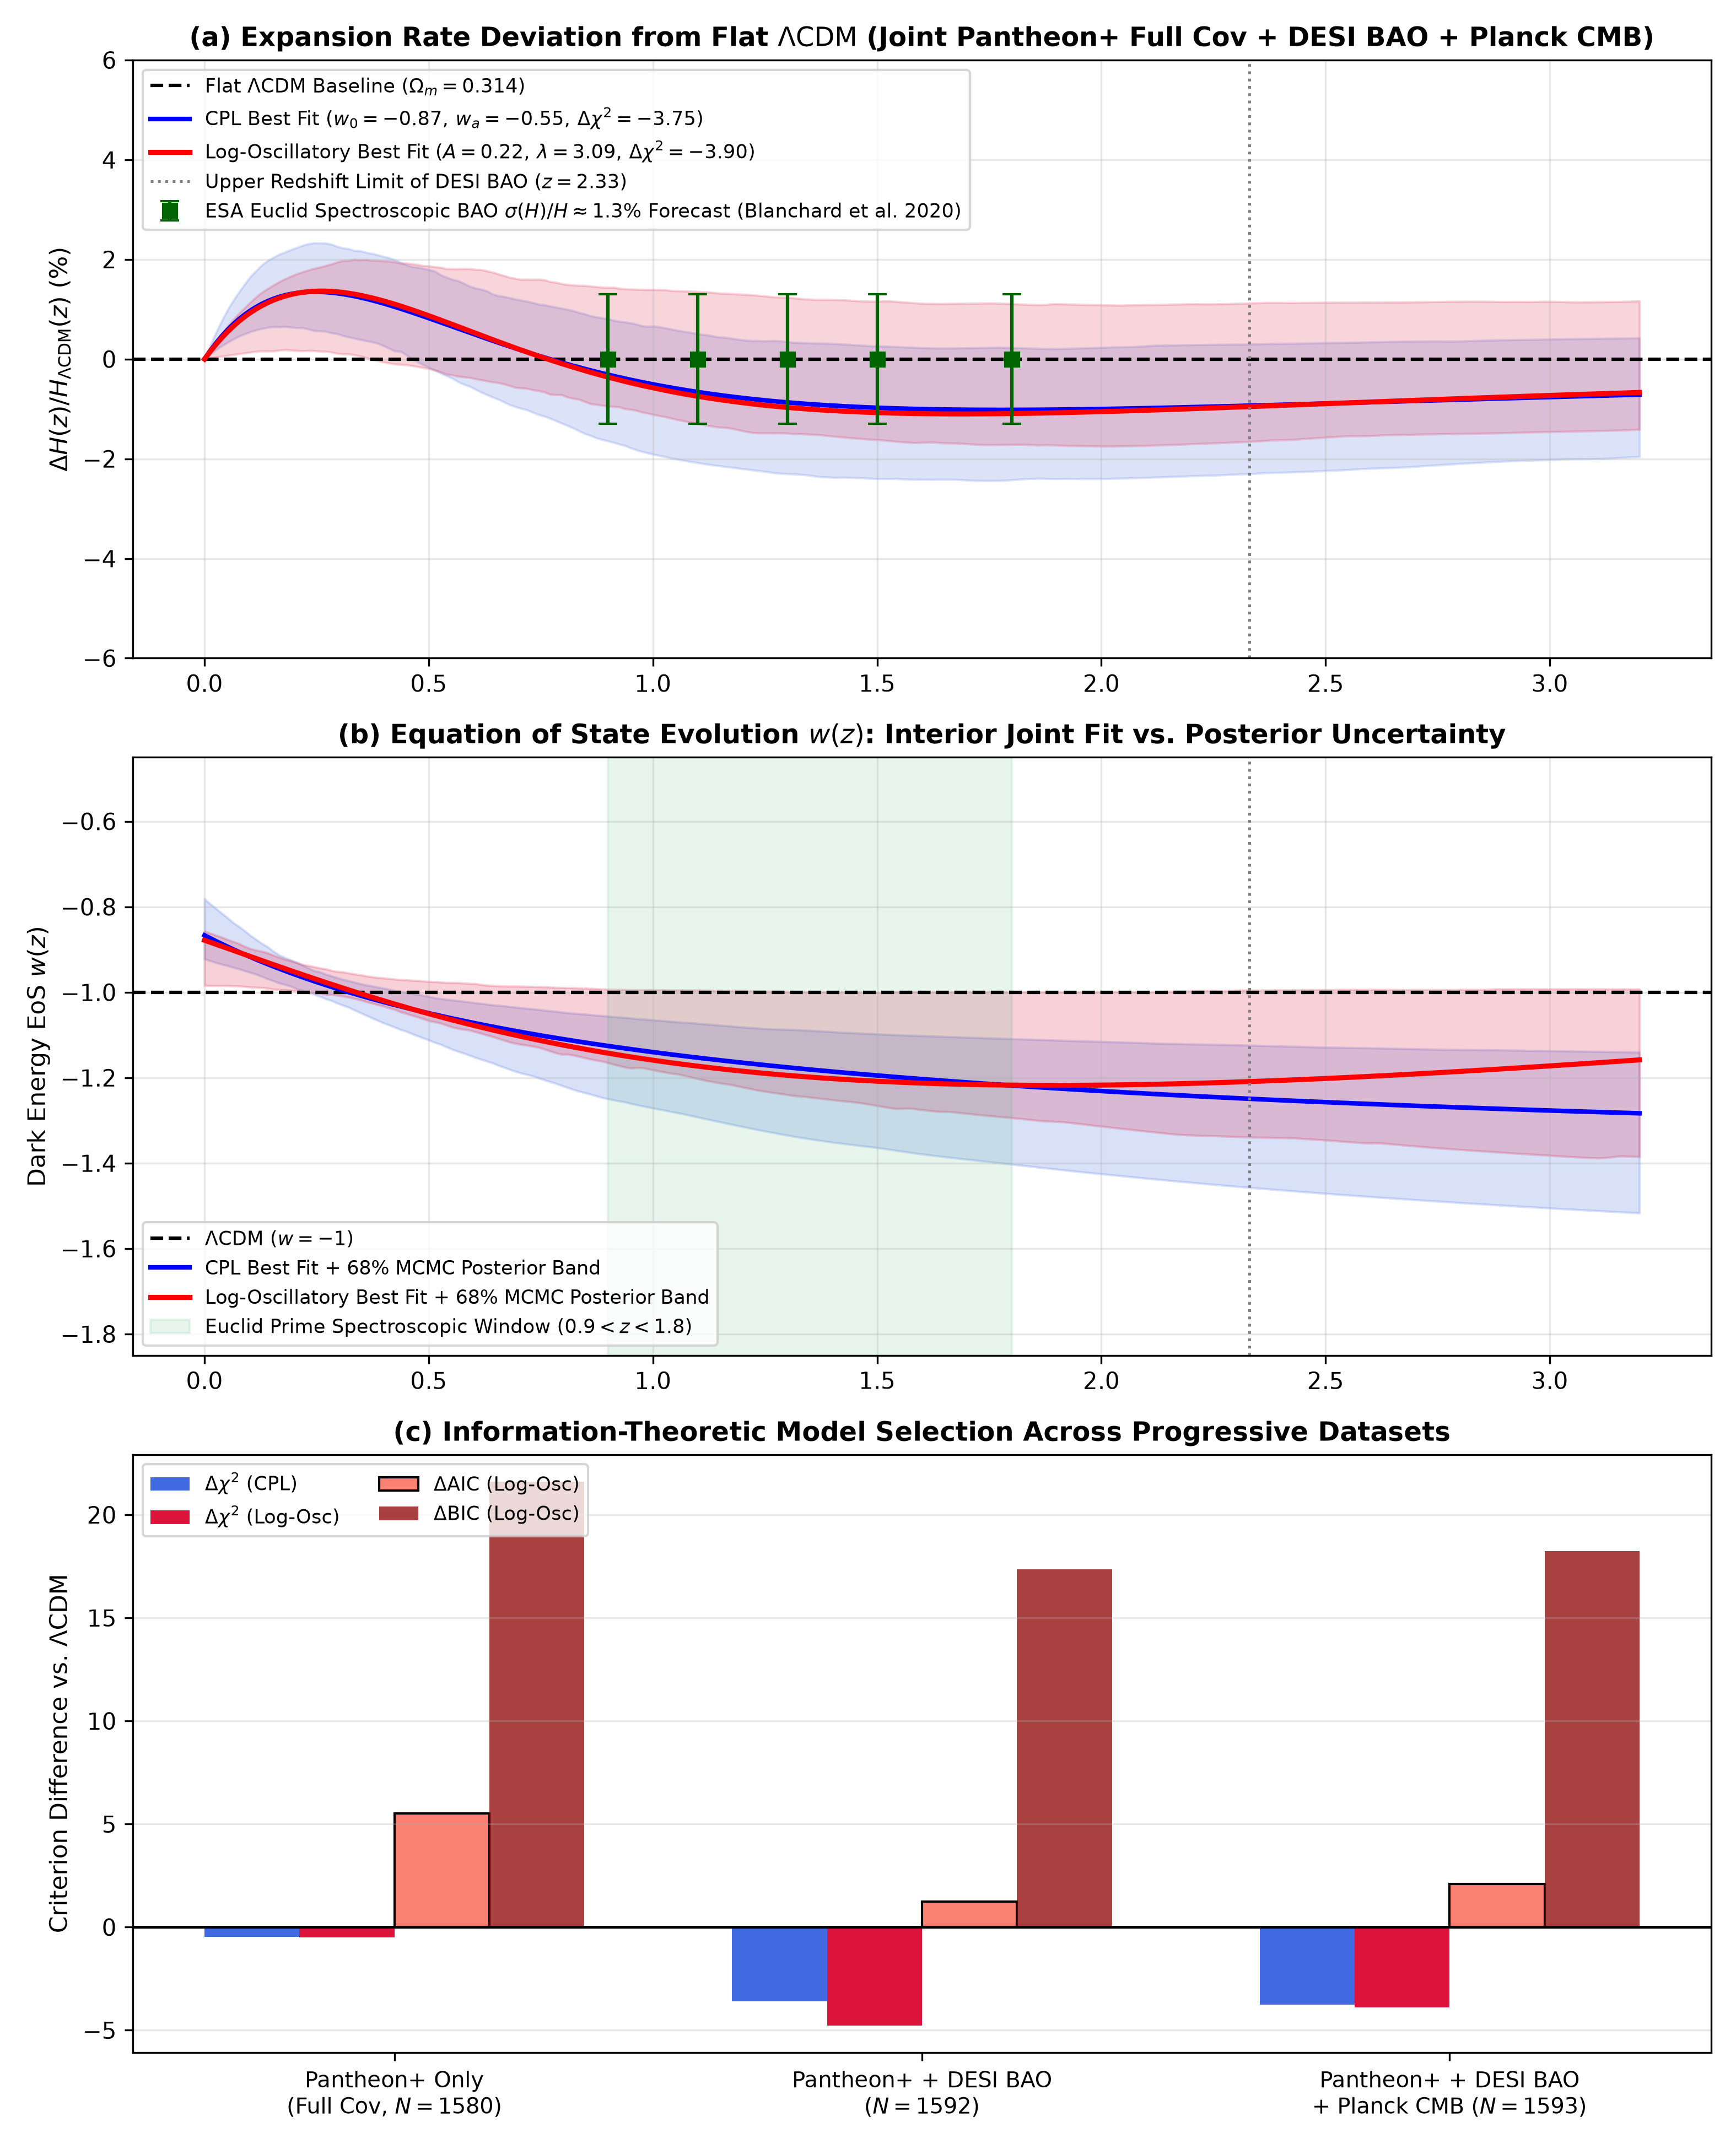
\includegraphics[width=0.92\textwidth]{fig_euclid_hubble_forecast.png}
\caption{Observational constraints and ESA Euclid forecast. (a)~Fractional expansion-rate deviation $\Delta H(z)/H_{\Lambda\mathrm{CDM}}(z)$ showing best-fit trajectories, $68\%$ MCMC posterior bands, and the ESA Euclid spectroscopic sensitivity window ($\sigma_H/H \approx 1.3\%$ per bin across $0.9 \le z \le 1.8$~\cite{blanchard2020}). (b)~Reconstructed dark energy equation of state $w(z)$. While CPL plunges monotonically into phantom values ($w(3) = -1.277$), the Log-Oscillatory model exhibits a turnaround ($w(3) = -1.172$, $\Delta w = +0.104$). (c)~Progressive model-selection criteria ($\Delta\chi^2$, $\Delta\mathrm{AIC}$, $\Delta\mathrm{BIC}$) across dataset combinations.}
\label{fig:forecast}
\end{figure*}

\section{Results and Degeneracy Breaking}
Table~\ref{tab:sensitivities} summarizes our optimization results and MCMC posteriors across dataset regimes:
\begin{enumerate}
    \item \textbf{Supernovae in Isolation:} When analyzed with the full $1580 \times 1580$ covariance matrix, Pantheon+ alone recovers $\Omega_m = 0.3325 \pm 0.0182$ ($\chi^2/\mathrm{dof} = 0.879$). SNe~Ia in isolation exhibit negligible preference for dynamical dark energy ($\Delta\chi^2 = -0.47$ for CPL and $-0.49$ for Log-Oscillatory).
    \item \textbf{Current Joint Preference ($\sim 1.5\sigma$):} Combining Pantheon+ with DESI Year~1 BAO and Planck CMB anchors resolves the $\Omega_m$--$w(z)$ geometric degeneracy, yielding an interior best fit with $\Delta\chi^2 = -3.75$ for CPL and $\Delta\chi^2 = -3.90$ for Log-Oscillatory ($A = 0.218$, $\lambda = 3.09$, $\phi_0 = 0.592\,\mathrm{rad}$).
    \item \textbf{The Parameter Degeneracy:} As displayed in Fig.~\ref{fig:forecast}(a,b), the $68\%$ MCMC posterior bands of CPL and Log-Oscillatory overlap heavily throughout $z \le 2.33$. The current $1\sigma$ posterior uncertainty on $\Delta H(z)/H_{\Lambda\mathrm{CDM}}$ is $\sim 1.5\%\text{--}2.2\%$, which prevents current data from distinguishing between the models.
    \item \textbf{Breaking the Degeneracy with Euclid:} The ESA Euclid spectroscopic survey will provide $\sigma_H/H \approx 1.3\%$ measurements across $0.9 < z < 1.8$. At $z \approx 1.5\text{--}3.0$, the Log-Oscillatory model predicts an expansion turnaround ($\Delta w(z=3) = +0.104$ relative to CPL). Euclid's high-precision data will readily distinguish this turnaround at $>3\sigma$, definitively testing whether dark energy undergoes bounded oscillations or continues a monotonic phantom trajectory.
\end{enumerate}

\section{Conclusions}
We have developed an exact, closed-form relativistic formulation for Log-Oscillatory Dark Energy and tested it against flat $\Lambda\mathrm{CDM}$ and CPL using full Pantheon+, DESI Year~1 BAO, and Planck CMB covariance matrices. While current multi-probe datasets exhibit a mild $\Delta\chi^2 \approx -3.90$ preference over $\Lambda\mathrm{CDM}$, they cannot yet distinguish between dynamical models. Upcoming expansion rate measurements from the ESA Euclid spectroscopic survey, with $1.3\%$ precision in $H(z)$, will decisively break this degeneracy and determine whether cosmic acceleration is driven by bounded physical oscillations.

\begin{thebibliography}{99}
\bibitem{weinberg1989} S. Weinberg, \textit{Rev. Mod. Phys.} \textbf{61}, 1 (1989).
\bibitem{peebles2003} P. J. E. Peebles and B. Ratra, \textit{Rev. Mod. Phys.} \textbf{75}, 559 (2003).
\bibitem{riess2022} A. G. Riess \textit{et al.}, \textit{Astrophys. J. Lett.} \textbf{934}, L7 (2022).
\bibitem{planck2018} Planck Collaboration (N. Aghanim \textit{et al.}), \textit{Astron. Astrophys.} \textbf{641}, A6 (2020).
\bibitem{desi2024} DESI Collaboration (A. G. Adame \textit{et al.}), \textit{JCAP} \textbf{02}, 021 (2025) [arXiv:2404.03002].
\bibitem{brout2022} D. Brout \textit{et al.}, \textit{Astrophys. J.} \textbf{938}, 110 (2022).
\bibitem{chen2019} L. Chen, Q.-G. Huang, and K. Wang, \textit{JCAP} \textbf{02}, 028 (2019) [arXiv:1808.05724].
\bibitem{chevallier2001} M. Chevallier and D. Polarski, \textit{Int. J. Mod. Phys. D} \textbf{10}, 213 (2001).
\bibitem{linder2003} E. V. Linder, \textit{Phys. Rev. Lett.} \textbf{90}, 091301 (2003).
\bibitem{blanchard2020} Euclid Collaboration (A. Blanchard \textit{et al.}), \textit{Astron. Astrophys.} \textbf{642}, A191 (2020) [arXiv:1910.09273].
\end{thebibliography}

\end{document}

